\begin{figure}[t]
    \centering
    \begin{subfigure}[b]{0.48\linewidth}
        \centering
        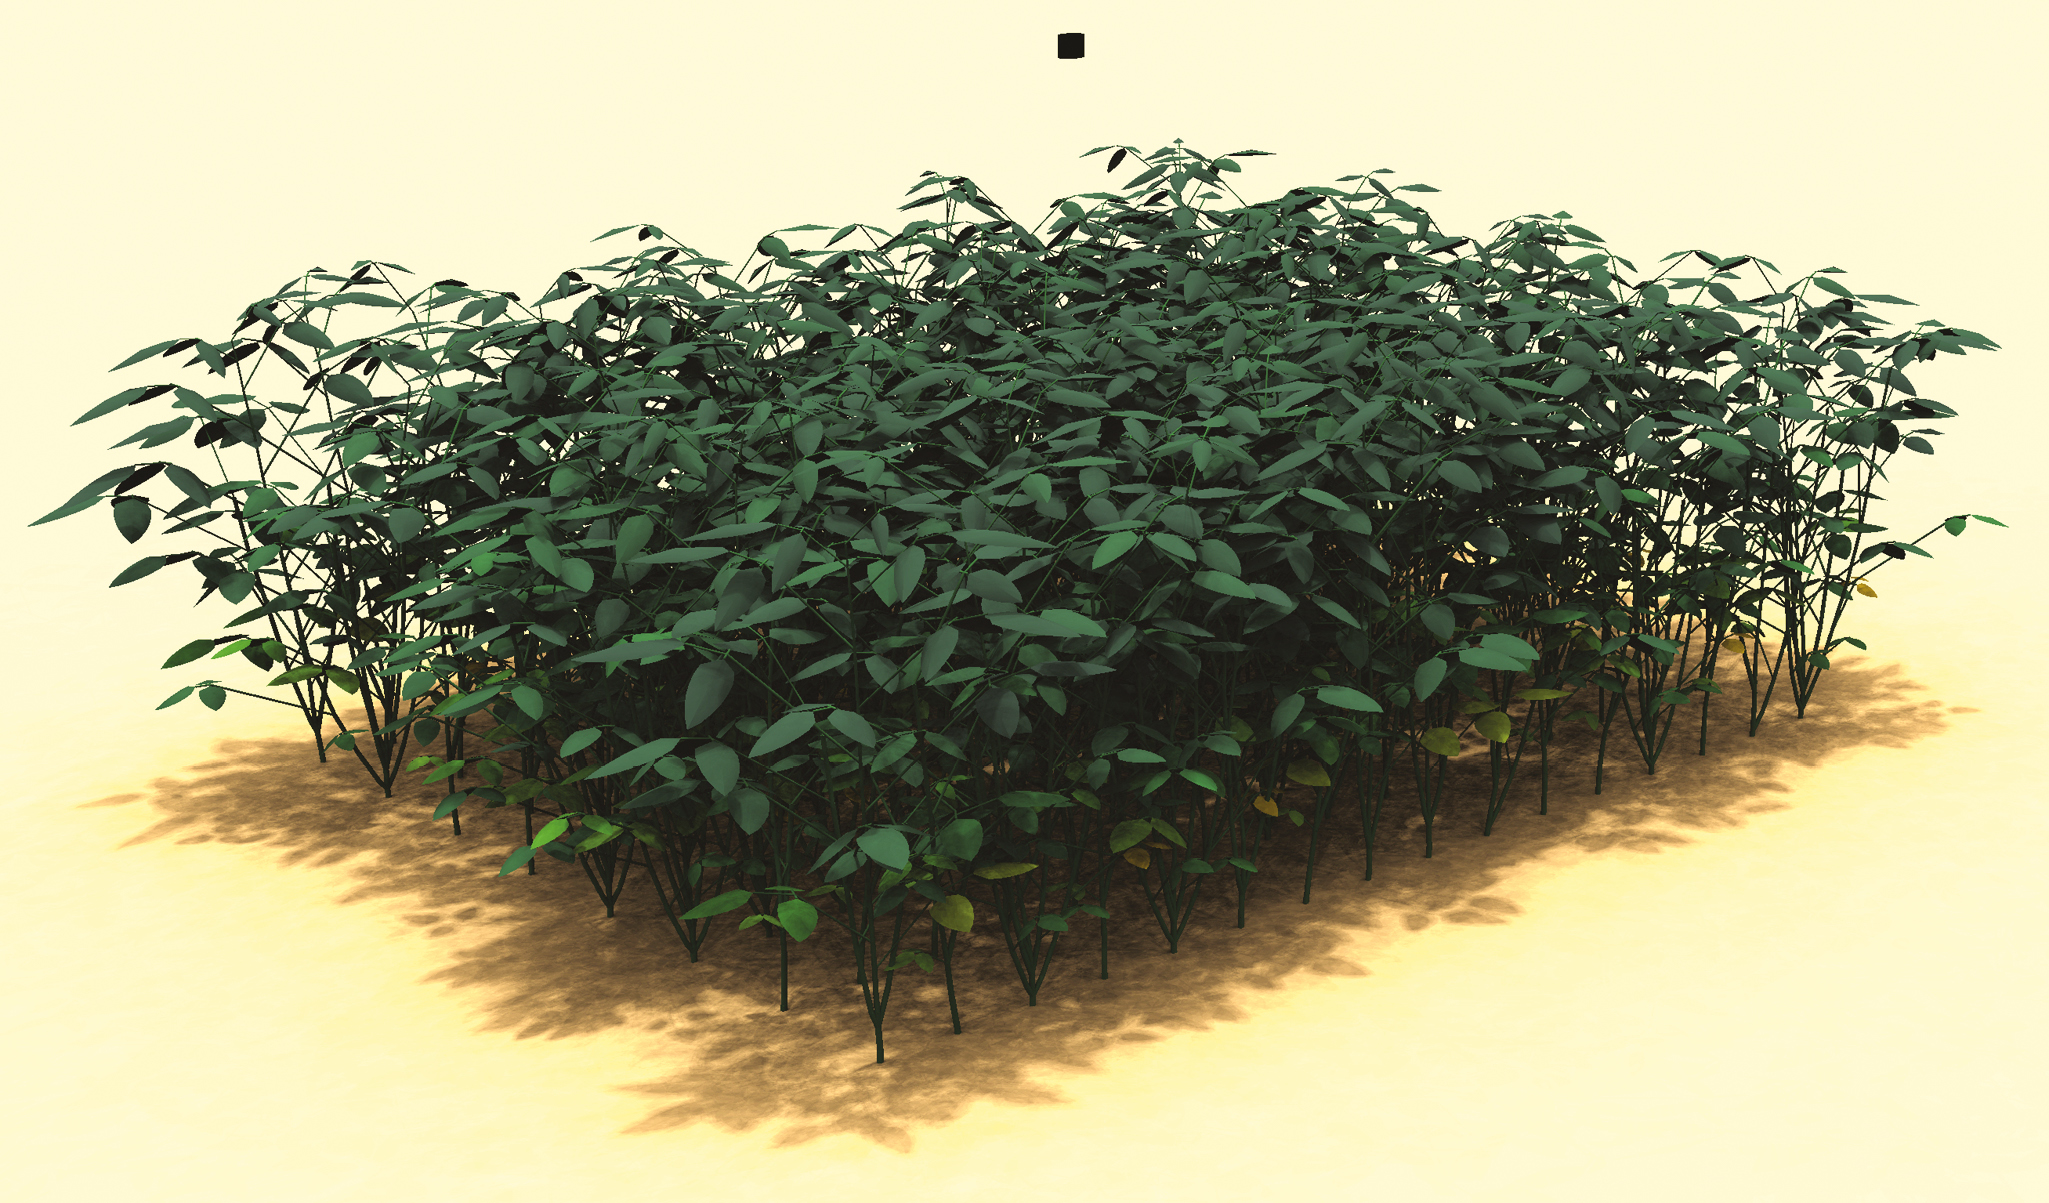
\includegraphics[width=\linewidth,height=\linewidth,keepaspectratio]{img/soybean_canopy_coussement.jpeg}
        \caption{Soybean FSPM}
        \label{fig:fspm-soybean-fspm}
    \end{subfigure}
    \hfill
    \begin{subfigure}[b]{0.48\linewidth}
        \centering
        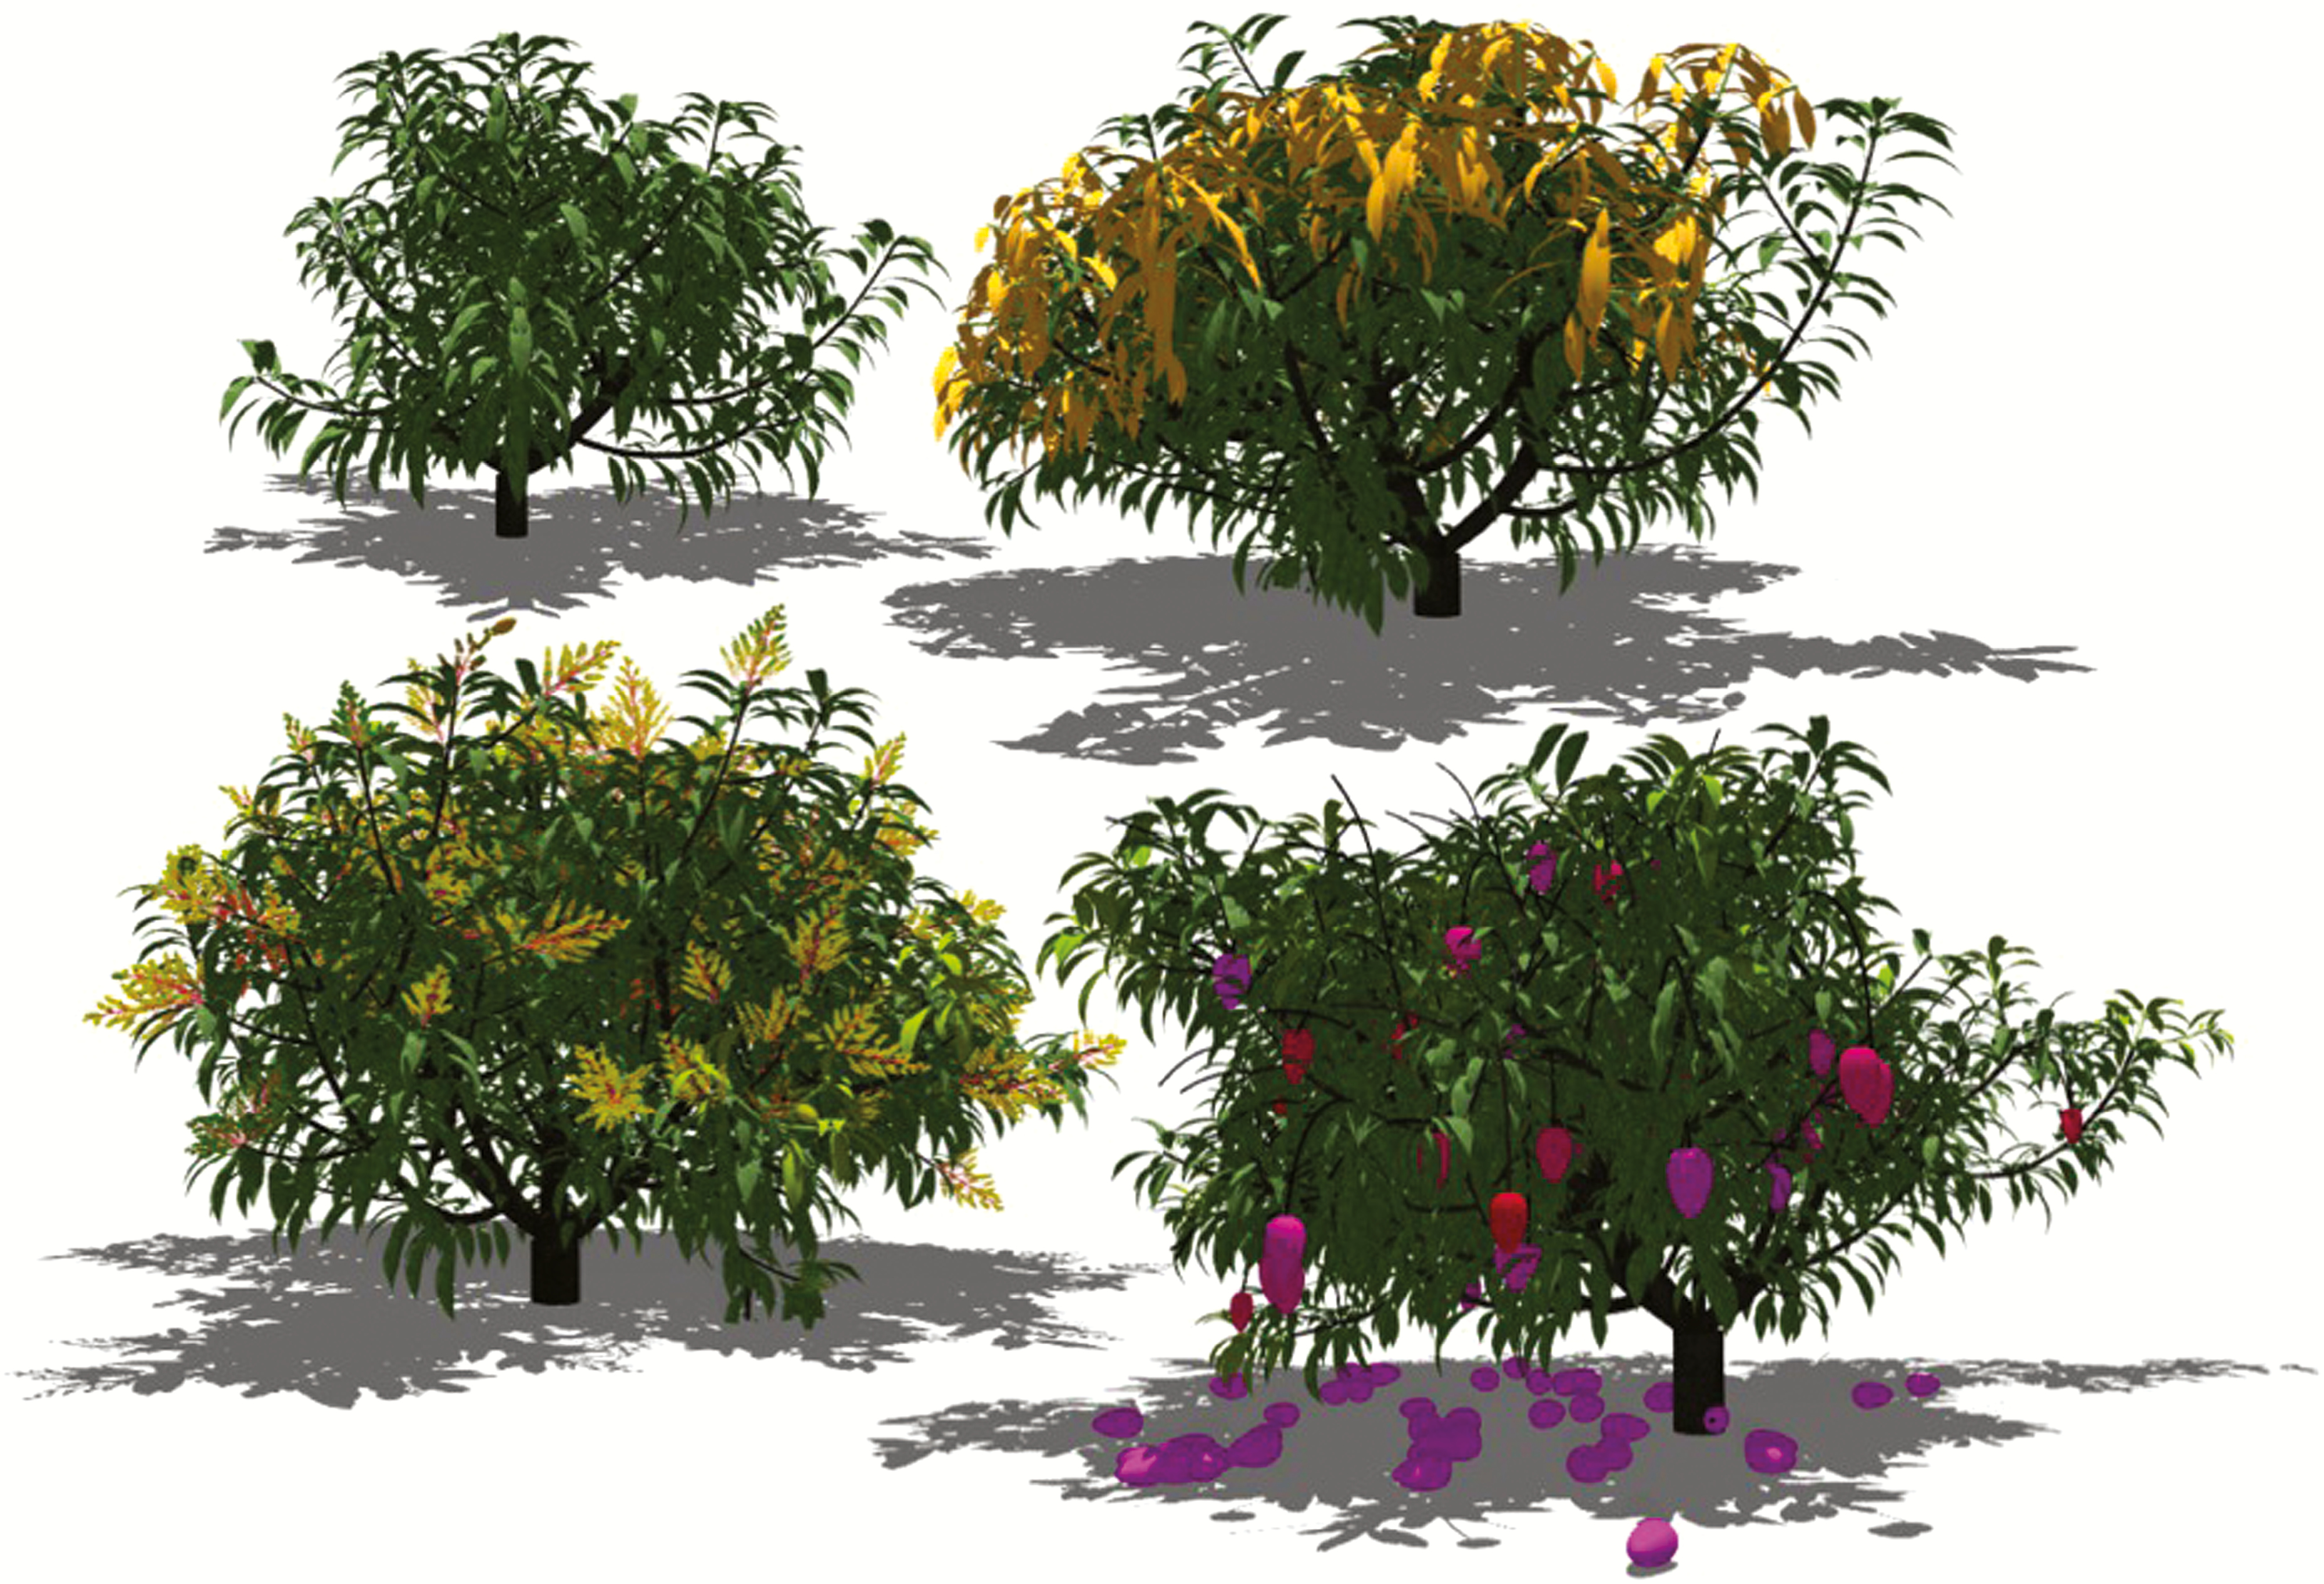
\includegraphics[width=\linewidth,height=\linewidth,keepaspectratio]{img/vmango_example.jpeg}
        \caption{V-Mango}
        \label{fig:fspm-vmango}
    \end{subfigure}
    % \vskip\baselineskip
    % \begin{subfigure}[b]{0.45\linewidth}
    %     \centering
    %     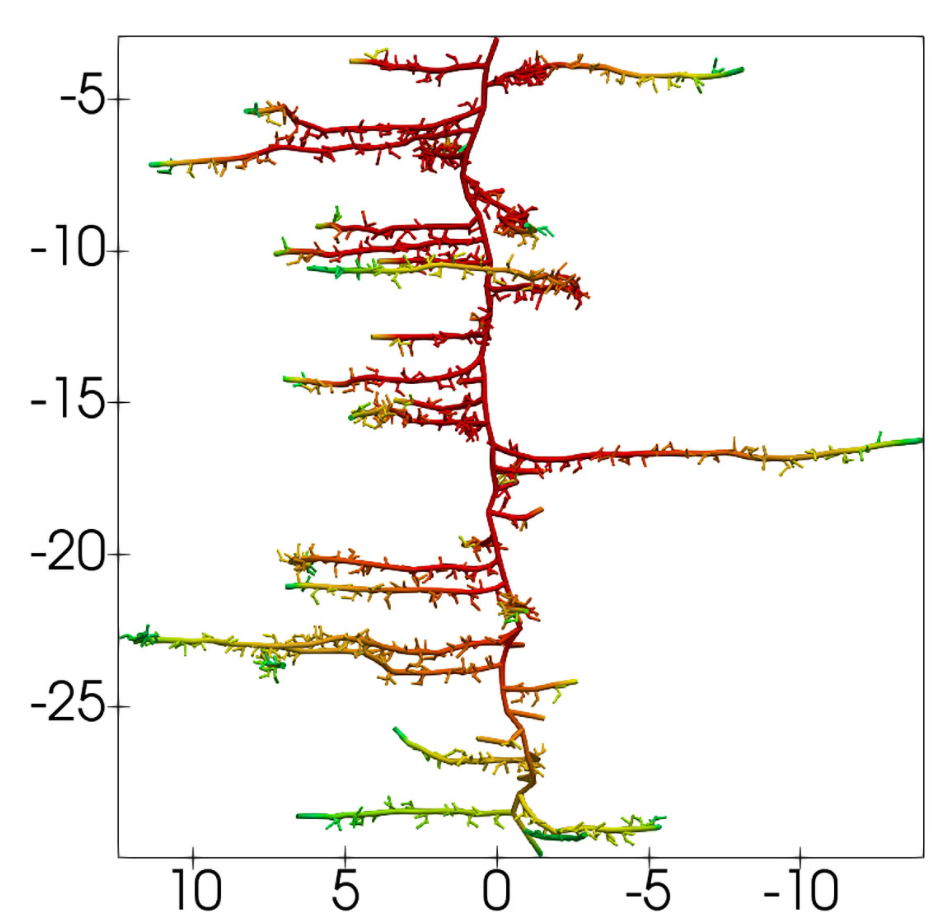
\includegraphics[width=\linewidth,height=\linewidth,keepaspectratio]{img/crootbox_example_anagallis_femina.png}
    %     \caption{CRootBox}
    %     \label{fig:fspm-crootbox}
    % \end{subfigure}
    % \hfill
    % \begin{subfigure}[b]{0.45\linewidth}
    %     \centering
    %     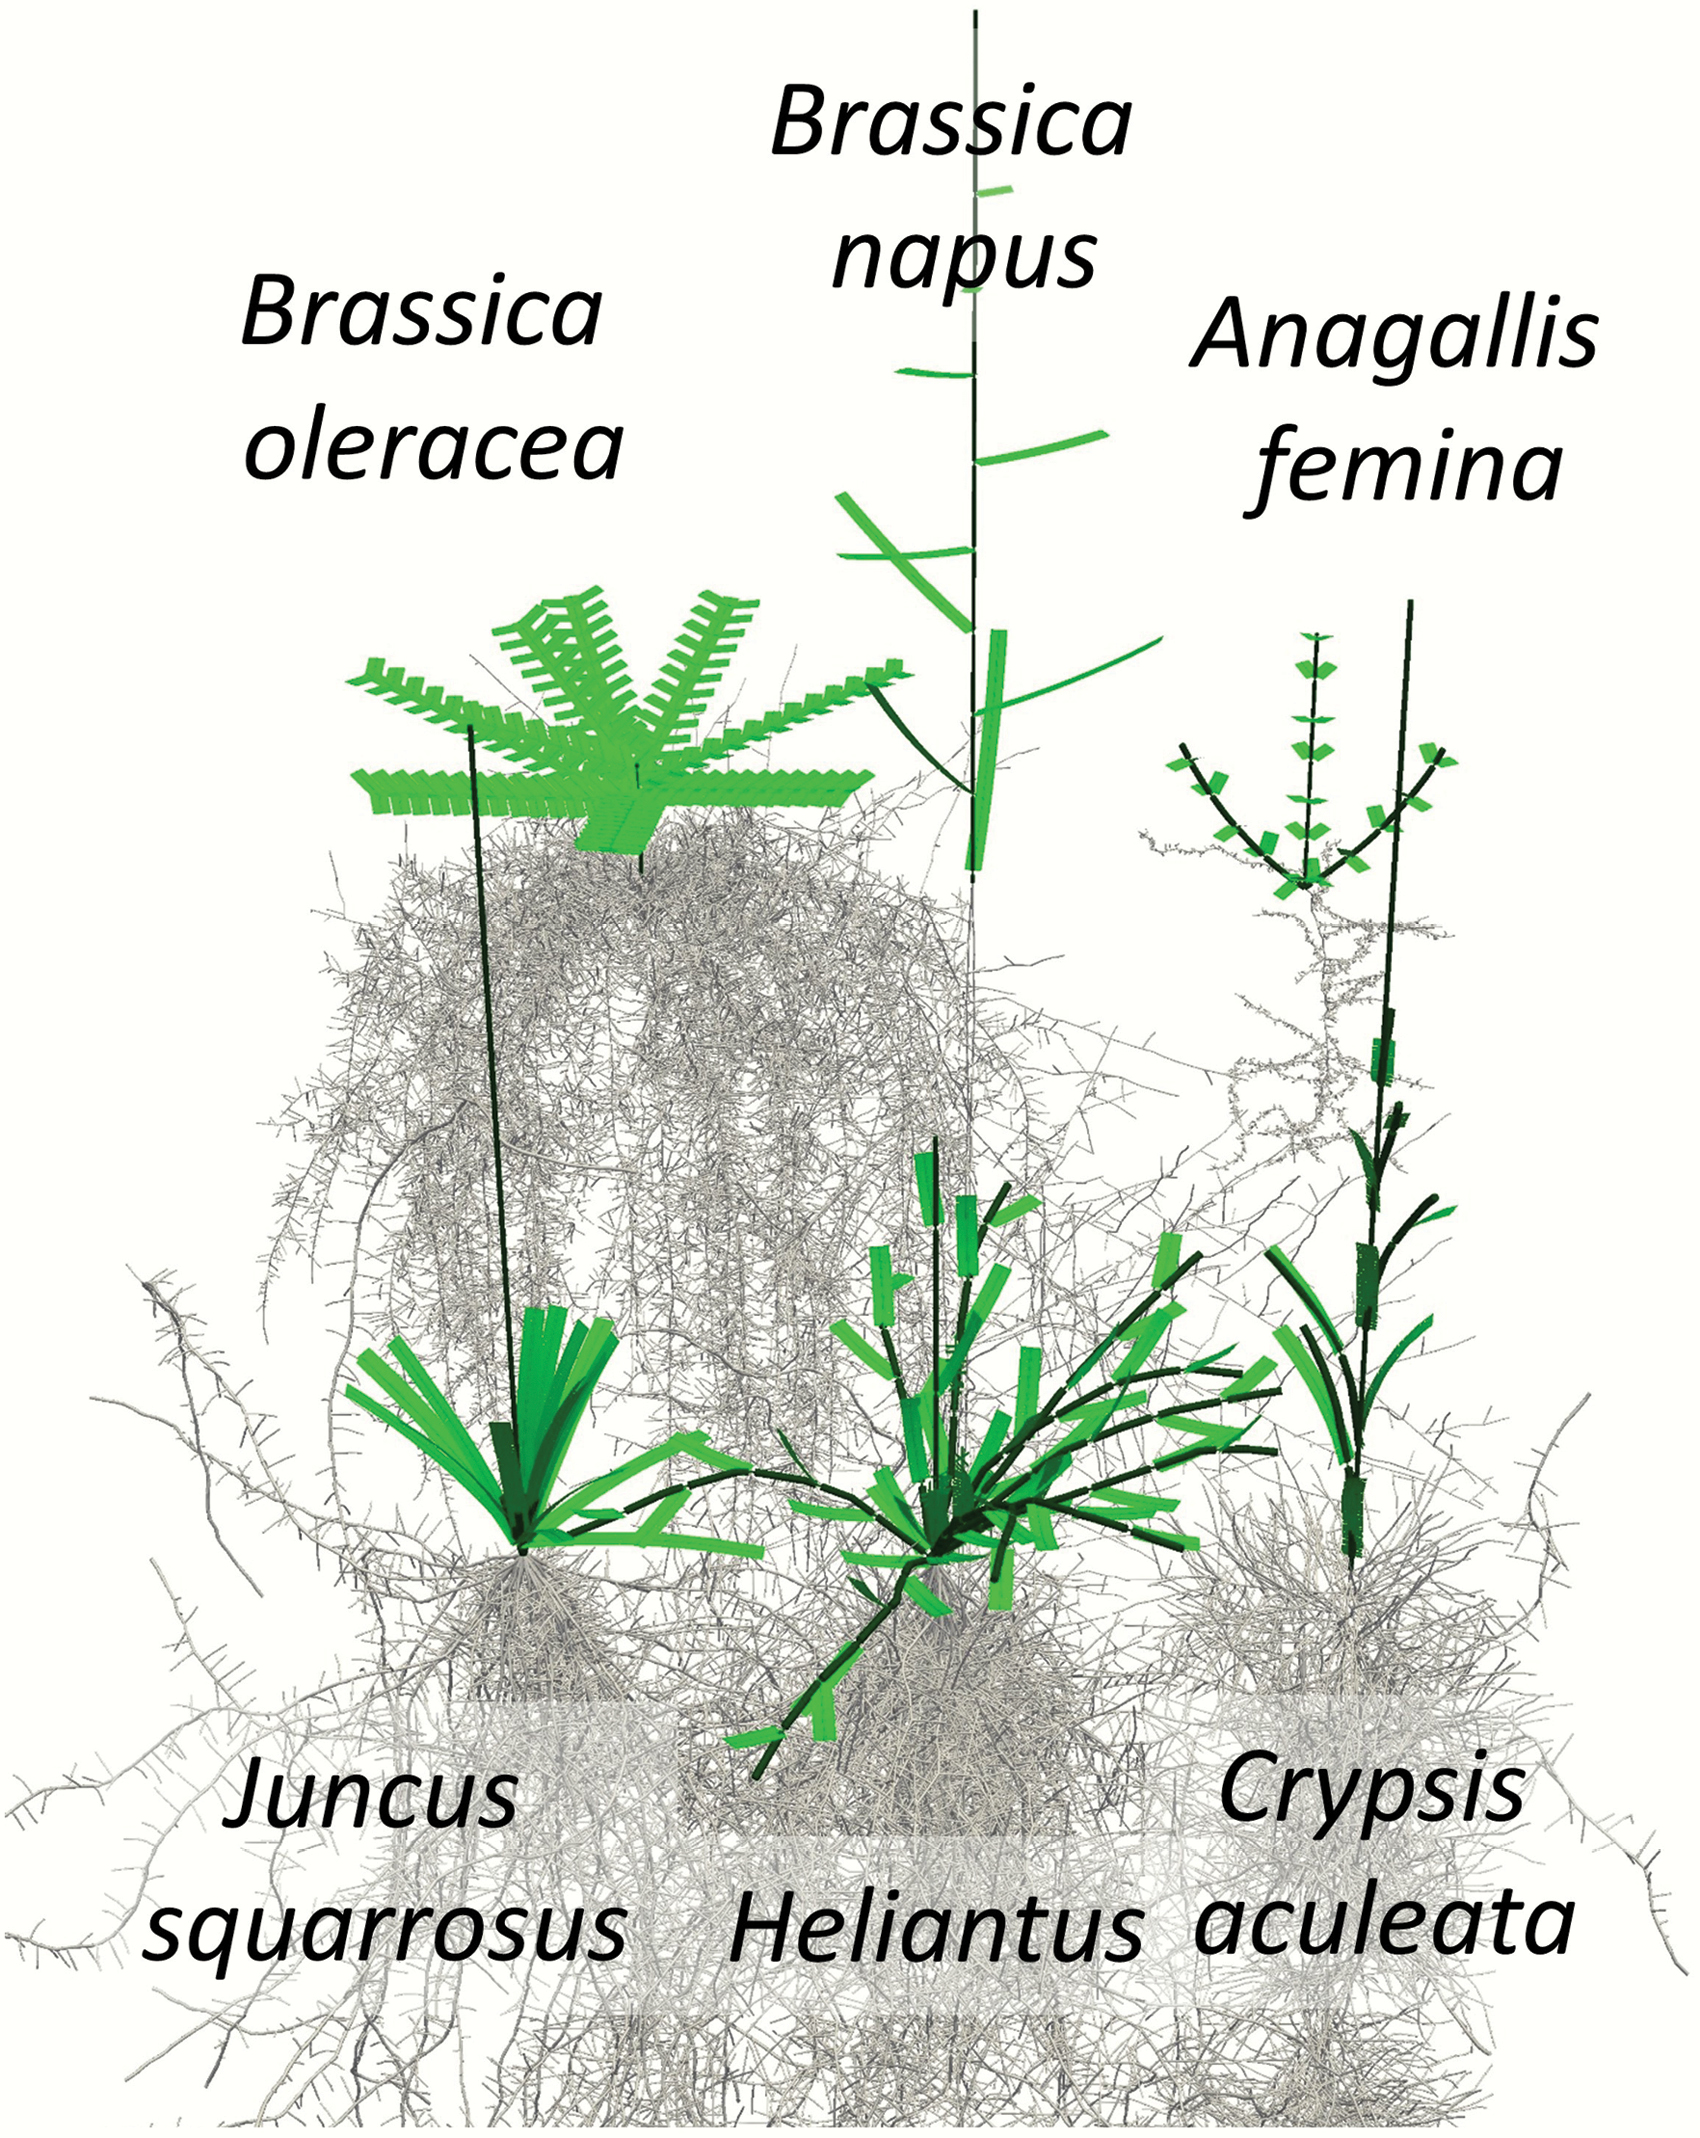
\includegraphics[width=\linewidth,height=\linewidth,keepaspectratio]{img/cplantbox_example.jpeg}
    %     \caption{CPlantBox}
    %     \label{fig:fspm-cplantbox}
    % \end{subfigure}
    \caption[Two examples of functional-structural plant models.]{
            Two examples of functional-structural plant models. 
            % (\subref{fig:fspm-soybean-fspm}) Soybean FSPM \supercite{coussement_turgor-driven_2020} is a highly detailed mechanistic plant growth model driven by hydrostatic pressure inside the plant cells. It also incorporates a ray-traced lighting model with dynamic lighting and shading conditions. 
            % (\subref{fig:fspm-vmango}) V-Mango \supercite{boudon_v-mango_2020} models the vegatative and reproductive development of mango trees to enable \textit{in silico} experimentation with better cultivation practices.
            % (\subref{fig:fspm-crootbox}) CRootBox \supercite{schnepf_crootbox_2018} is a generic framework for modeling the growth of plant roots in varying soil and environmental conditions.
            % (\subref{fig:fspm-cplantbox}) CPlantBox \supercite{zhou_cplantbox_2020} is built on top of CRootBox to provide a generic framework for modeling plant architecture and growth. It can be coupled with existing simulations of eco-physiological processes to create mechanistic plant models. 
            Figures originally appeared in their respective cited works.
            (\subref{fig:fspm-soybean-fspm}) Soybean FSPM \citep{coussement_turgor-driven_2020}. Figure reused with permission from the publisher (Copyright 2018 Oxford University Press).
            (\subref{fig:fspm-soybean-fspm}) V-Mango \citep{boudon_v-mango_2020}. Figure reused under the CC BY 4.0 license.
    }
    \label{fig:plant_model_examples}
\end{figure}

% (Coussement et al. 2018\supercite{coussement_modelling_2018})
